\documentclass[10pt]{article}
\usepackage[usenames]{color} %used for font color
\usepackage{amssymb} %maths
\usepackage{amsmath} %maths
\usepackage[ruled,linesnumbered]{algorithm2e}
\usepackage[utf8]{inputenc} %useful to type directly diacritic characters

\usepackage{graphics}
\usepackage{adjustbox}
\usepackage{float}
\begin{document}
\begin{raggedright}
Michael Lan \\
Lingfei Zeng \\
Xunjie Zhu \\
\end{raggedright}

\vspace{5mm} 

Stage2 - The Design Stage. 
\begin{itemize} 
\item{ Design Description:\\} 
\begin{itemize}
The user is given 3 different similarity measures for searching. We will begin with the first similarity measure, which allows users to find tweets clusters related to search term inputs.
(Search phrase and retrieve tweets with similar phrases acc to edit distance)

\item[$\diamond$]{\bf1) Tweet clustering based on semantic similarity}

We aim to cluster tweets into different groups using Hierarchical Clustering. To do this, we require semantic similarity scores. We compute these using the extended {\bf Edit Distance} algorithm integrated {\bf Word2Vec} embedding to compute the distance between sentences in the tweets, and by grouping by shortest distance we divide tweets into different groups. \\\\
In details, we describe tweet sentence $S_1$ as $S_1$=\{$a_1$,$a_2$,…,$a_n$\} and sentence $S_2$ as $S_2$ =\{$b_1$,$b_2$, …,$b_m$\}. $S_1$ consists of n words and $S_2$ consists of m words. $a_i$ is the i th word of $S_1$ and $b_j$ is the j th word of $S_2$. We use Sim($S_1$,$S_2$) to describe the similarity between $S_1$ and $S_2$, with the range of 0 (no relation) to 1 (semantic equivalence). For edit distance, we utilize Levenshtein Distance algorithm to extend to the word sets in sentences. We define the Levenshtein distance between $S_1$ and $S_2$ is L(n,m), where  \(0\leq i\leq n\) and \(0\leq j\leq n\). And we have: \[L(i, j) = max(i, j)  \qquad   if \quad min(i,j)=0, \]  

$$
L(i, j) = min
\left\{
\begin{array}{ll}
L(i-1, j-1) + c(a_i,b_j) \\
L(i, j-1) +1 \\
L(i-1, j) +1
\end{array}
\right.
otherwise.
$$
Where the function c($a_i$,$b_j$) is defined as
$$
c(a_i, b_j)=
\left\{
\begin{array}{ll}
0 \quad (a_i = b_j) \\
1 \quad (a_i \neq b_j)
\end{array}
\right.
$$

We also need to consider the circumstances that if two different words have the same or similar meaning (e.g., “cat” and “kitty”), in which case edit distance defines them as a mismatch. We address this issue by introducing Word2vec to measure semantic similarity between words. 
%{\sf Word2vec}~\cite{word2vec} 
Word2vec [1] is an unsupervised  deep learning algorithm that maps each word to a vector  $\in \mathcal{R}^n$ such that the semantically similar words are mapped to the vectors that are close to each other in the geometry space. 
In our settings, given any two words, e.g.,  $a_i$ and $b_j$ in the above, we first apply word2vec to map them to two vectors, $\vec{v}_1$ and $\vec{v}_2$, and then use the euclidean distance, $\lVert \vec{v}_1 - \vec{v}_2 \rVert$, to measure the cost of the replacement.
We may normalize the cost into a relatively small range. 

$$
\begin{array}{c}
c(a_i, b_j)=\lVert \vec{v}_1 - \vec{v}_2 \rVert \\
 where \quad  \vec{v}_1 = word2vec(a_i), \vec{v}_2=word2vec(b_j)
\end{array}
$$

\item[$\diamond$]{\bf 2a) Recommending tweets and hashtags based on network similarity}\\

Next, we will describe searching by network similarity. Users can input either a tweet or a hashtag to find similar tweets and hashtags from the stored data. If the data does not contain those search terms, the user can choose to 'Gather New Tweets' based on
the search terms. \\

A directed bipartite network G with two different types of nodes, tweets and hashtags, will be created. Instead of storing nodes as strings, we give a unique ID to each node. A tweet will have an outgoing edge to a hashtag if it contains it. The graph $ G^2$ has as its nodes every pair of tweets and every pair of hashtags in G. As explained below, we will prune these node pairs to get an array called computed\_pairs. In Algorithm 3, we apply SimRank on computed\_pair  to find a similarity score for every pair of nodes which are not 'far apart', a subjective measure. \\

SimRank, shown in Algorithm 3, is calculated using these equations: Let A and B be tweets. O(v) are the outgoing neighbors of v. The similarity s(A,B) is:

$$s(A,B) = \dfrac{C\textsubscript{1}}{|O(A)||O(B)|} \sum_{i=1}^{|O(A)|} \sum_{j=1}^{|O(B)|} s(O\textsubscript{i}(A),O\textsubscript{j}(B))$$

C is a constant between 0 and 1. It is the decay factor and is the only adjustable parameter of the algorithm; we will set it as 0.8. \\

Let c and be be hashtags. I(v) are the ingoing neighbors of v.  The similarity s(c,d) is:

$$s(c,d) = \dfrac{C\textsubscript{2}}{|I(c)||I(d)|} \sum_{i=1}^{|I(c)|} \sum_{j=1}^{|I(d)|} s(I\textsubscript{i}(c),I\textsubscript{j}(d))$$

The similarity between two nodes is the average similarity of their neighbor. Initially, for node x, all node pairs (x,x) have score 1, while other node pairs have score 0. Next, the similarity scores are calculated according to the equations above. This step is iterated until the updated scores do not differ much from the previous iteration. Since s(a,b) and s(b,a) are symmetric, so only need to store one of their scores. More information can be found in the original paper, the powerpoints, or by contacting this report’s authors. \\

For memory efficiency, pairs of nodes which are far away are pruned out. Let M be the adjacency matrix of G. If entry (n,m) in $M^k$ is nonzero, then there exists a path between n and m of length k. Let Kmax be a subjective upper bound; we will set it as 4. Consider:
$$Z = \sum_{k=1}^{Kmax} M^{2k}$$

Only even powers of M are included in Z because G is bipartite. Then we will only compute similarity scores on the nonzero entries of Z, which are gathered into computed\_pairs.
\\

\item[$\diamond$]{\bf 2b)Time and Space Complexity for pruning node pairs and running SimRank}\\

The bulk of the running time depends on the matrix multiplication used to obtain computed\_pairs; this takes $\Theta(n^3)$. The second pruning approach, computing the shortest path for all pairs, takes $O(n\log{}n)$ for each pair, and since there are $ n^2$ pairs, its total running time would be $O(n^3\log{}n)$. Thus, the adjacency matrix multiplication approach is preferred. \\

Now let d = the average of $|I(a)|*|I(b)|$ over all nodes in $ G^2$ . Let K = average number of iterations the algorithm performs. Let w be the number of pairs in computed\_pairs . Using a ‘naive’ implementation of SimRank, average running time of Algorithm 3 is O(K*w*d). Its worst case mainly depends on K. We store node\_scores in a hash table, so its space complexity is O(n).\\\\\\\\

\end{itemize}

\begin{figure}[H]
  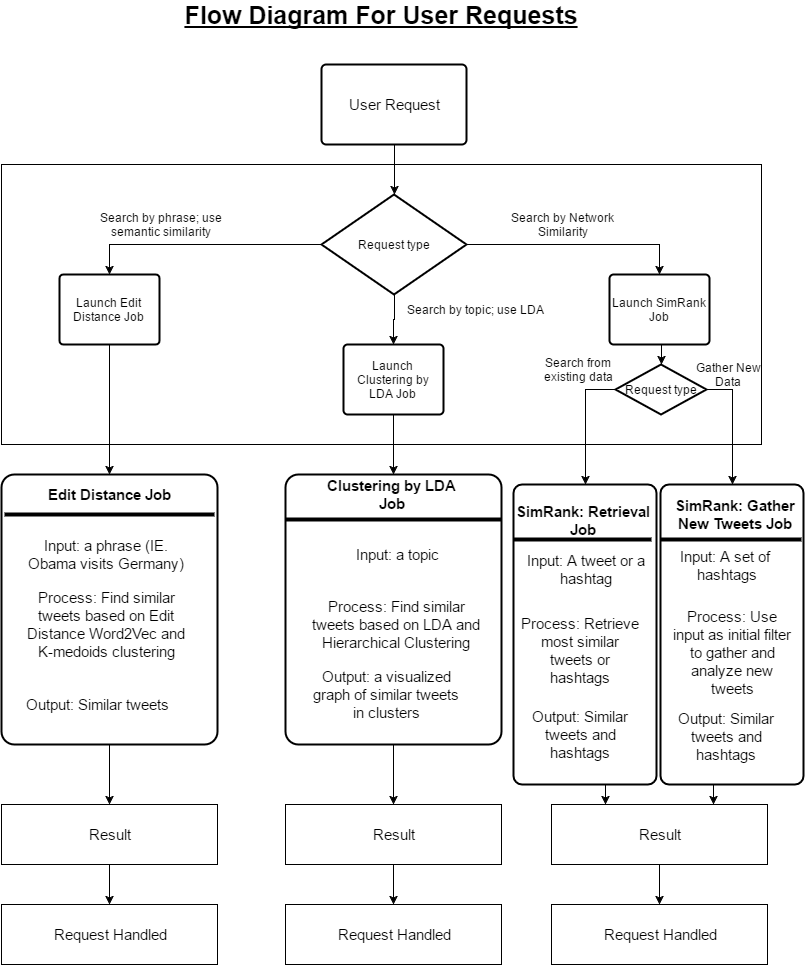
\includegraphics[width =\linewidth]{UI flowchart.png}
\end{figure}

\pagebreak

\item{\bf High Level Pseudo Code}

  \scalebox{0.75}{
    \begin{minipage}{0.7\linewidth}
\begin{algorithm}[H]
	\SetKwData{Left}{left}
	\SetKwData{This}{this}
	\SetKwData{Up}{up}
	\SetKwFunction{Union}{Union}
	\SetKwFunction{FindCompress}{FindCompress}
	\SetKwInOut{Input}{input}
	\SetKwInOut{Output}{output}
	\Input{A sentence $S_1$ with n words as $S_1$=\{$a_1$,$a_2$,…,$a_n$\} and a sentence $S_2$ with m words $S_2$ =\{$b_1$,$b_2$, …,$b_m$\} }
	\Output{The edit distance between $S_1$ and $S_2$ L(n,m)}
	\BlankLine
	\emph{}\
	\For{$i = 0$ to n}{
		L($i, 0$) = $i$	
	}
    \For{$j = 0$ to m}{
	    L($0, j$) = $j$	
    }

    \For{$i = 1$ to n}{
    	\For{$j = 1 $to m} {
    			L($i, j$) = min \{L($i-1, j$) +1, L($i, j-1$) +1, L($i-1, j-1$) + c($a_i, b_j$)\} 
    		}
    } 
    return L(m, n)	
	
	\caption{Edit Distance}\label{algo_disjdecomp}
\end{algorithm}
\end{minipage}%
    }

  \scalebox{0.75}{
    \begin{minipage}{0.7\linewidth}
\begin{algorithm}[H]
	\SetKwData{Left}{left}
	\SetKwData{This}{this}
	\SetKwData{Up}{up}
	\SetKwFunction{Union}{Union}
	\SetKwFunction{FindCompress}{FindCompress}
	\SetKwInOut{Input}{input}
	\SetKwInOut{Output}{output}
	\Input{An integer n represents the number of initial clusters, a clusterMatrix stores the sentence vector of every cluster, an array, a queue(implemented by binary heap) stores indices and distances between two cluster}
		\Output{clustered nodes}
	    \For{$i = 1$ to n}{
	    	initiaDistance($i, i$) = 0\;
	    	\For{$j = i+1 $to n} {
			initiaDistance($i, j$) = distance($i, j$)
    			queue add entry(initiaDistance($i, j$), i, j, 1, 1)
		}
    } 
      \While{$n \geq miniumClusters$} {
      	entry = queue.pop()\;
	merge(entry.cluster1, entry.cluster2, entry.distance, entry.distance, clusterMatrix)\;
		    \For{i = 1 to n}{\
		    \If{$i \neq entry.cluster1 and clusterMatrix[i].size \neq 0 $}{
		    $first = min(entry.cluster1, i)$\;
		    $second = min(entry.cluster2, i)$\;
		    newDistance = getDistance(initialDistance, clusterMatrix(first), clusterMatrix(second))\;
		    queue add entry(newDistance, first, second, clusterMatrix(first).size, clusterMatrix(second).size)
		    }
	}
			    n = n -1;
      }
	\BlankLine
	\emph{}\
		
\caption{Hierarchical Clustering Algorithm}\label{algo_disjdecomp}
\end{algorithm}
\end{minipage}%
    }

  \scalebox{0.75}{
    \begin{minipage}{0.7\linewidth}
\begin{algorithm}[H]
	\SetKwData{Left}{left}
	\SetKwData{This}{this}
	\SetKwData{Up}{up}
	\SetKwFunction{Union}{Union}
	\SetKwFunction{FindCompress}{FindCompress}
	\SetKwInOut{Input}{input}
	\SetKwInOut{Output}{output}
	\Input{An array of node pairs called computed\_pairs }
	\Output{A hash table of similarity scores for every node pair in computed\_pairs}
	\BlankLine
	\emph{}\
	Create hash table node\_scores\;
	\For{(a,b) in nodes(G\_2):}{
		\eIf{a==b}
			{Node\_scores[(a,b)] := 1}
			{Node\_scores[(a,b)] := 0}
	}
	stop\_signal := off\;
	\While{stop\_signal == off}{
		stop\_signal := on\;
		\For{(a,b) in nodes(G\_2)}{
			\If{a != b}
				{\{COMMENT: Let N(v) denote the neighbors of node v \} \\
				R\textsubscript{k}(a,b) := $$\dfrac{C\textsubscript{1}}{|N(a)||N(b)|} \sum_{i=1}^{|N(a)|} \sum_{j=1}^{|N(b)|} R\textsubscript{k-1}(N\textsubscript{i}(a),N\textsubscript{j}(b))$$}
			\If{$ | R\textsubscript{k}(a,b) - R\textsubscript{k-1}(a,b) | > 0.05$}
				{stop\_signal := off}
			node\_scores[(a,b)] := R\_k(a,b) 
		}
	}
	Return node\_scores
	\caption{Node pair similarity scores pseudocode}\label{algo_a}
\end{algorithm}
\end{minipage}%
    }

\item{\bf Algorithms and  Data Structures:}
In Algorithm 1, the major algorithm is Edit Distance in Dynamic Programming. The data structure is two-dimensional array, and the time complexity is $ \mathcal{O}(mn)$. In Algorithm 2, we use Agglomerative Hierarchical Clustering Algorithm to cluster the documents. The time complexity of this algorithm is $ \mathcal{O}(n^2logn)$. In Algorithm 3, the nodes with their IDs are stored in hash tables. The graphs, represented as adjacency lists, are also stored in hash tables. The node pairs and their scores are stored in hash tables. Similar tweets and hashtags are stored in arrays. \\
\end{itemize}

\iffalse
\begin{itemize} 
\item{  Flow Diagram Major Constraints.}
Please insert here the integrity constraints:
\begin{itemize} 
\item{ Integrity Constraint. }
Please insert the first integrity constraint in here together with its description and justification. 
\end{itemize}
Please repeat the pattern for each integrity constraint.
\end{itemize}
\fi



%\bibliographystyle{abbrv}
%\bibliography{stage2_new}  % sigproc.bib is the name of the Bibliography in this case

\begin{thebibliography}{2}
%\iffalse
\bibitem{edit}
T. Mikolov, I. Sutskever, K. Chen, G. Corrado, and J. Dean. Distributed
representations of words and phrases and their compositionality. In Proceed-
ings of the 26th International Conference on Neural Information Processing
Systems, NIPS'13, pages 3111-3119, USA, 2013. Curran Associates Inc.
%\fi
	
\bibitem{simrank} 
Jeh, Glen, and Jennifer Widom. "SimRank: a measure of structural-context similarity." In Proceedings of the eighth ACM SIGKDD international conference on Knowledge discovery and data mining, pp. 538-543. ACM, 2002.

\end{thebibliography}

\end{document}
